\documentclass[11pt]{standalone}
\usepackage{amssymb}
\usepackage{amsmath}
\usepackage[no-math]{fontspec}
\usepackage{unicode-math}
\usepackage{libertinus}
\usepackage{pgf,xcolor}
\usepackage{tikz}
\usetikzlibrary{arrows.meta, backgrounds}
\usepackage{pgfplots}
\pgfplotsset{compat=newest}

\definecolor{my_darkgray}{HTML}{484949}
\definecolor{my_lightgray}{HTML}{F3F4F4}
\definecolor{my_darkblue}{HTML}{005A94}
\definecolor{my_lightblue}{HTML}{CCDEE9}
\definecolor{my_yellow}{HTML}{FFEC7F}
\definecolor{my_red}{HTML}{E60000}
\definecolor{my_orange}{HTML}{E87846}

\begin{document}
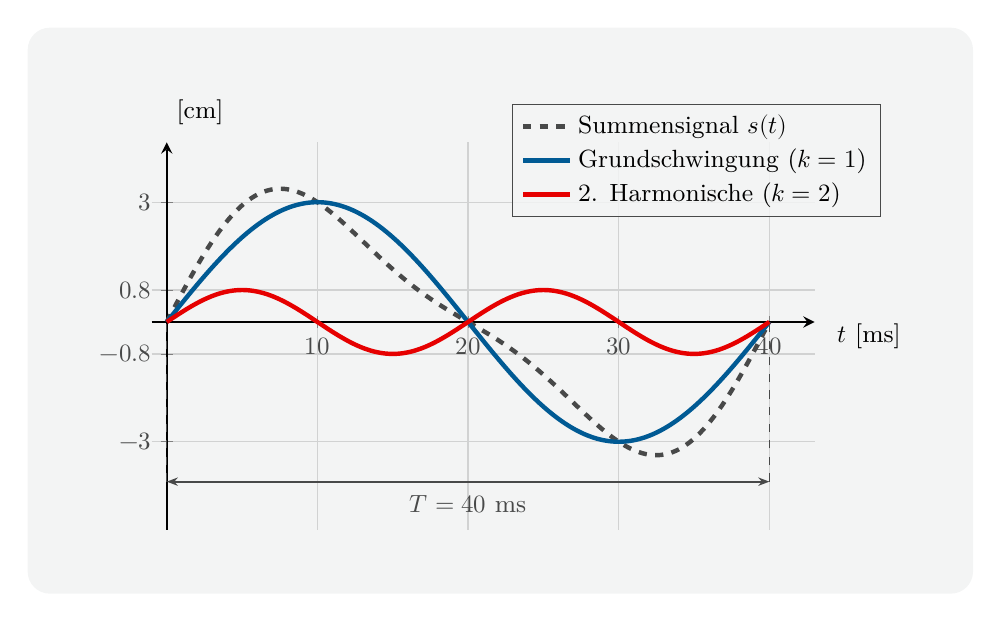
\begin{tikzpicture}[
    show background rectangle,
    background rectangle/.style={fill=my_lightgray, rounded corners=8pt},
    inner frame sep=0.8cm
]

\begin{axis}[
    axis lines = center,
    xlabel = {$t$ [ms]},
    ylabel = {[cm]},
    xlabel style={at={(axis description cs:1.02,0.5)}, anchor=west, font=\small},
    ylabel style={at={(ticklabel* cs:1.02)}, anchor=south west, font=\small},
    xmin = -1,
    xmax = 43,
    ymin = -5.2,
    ymax = 4.5,
    xtick = {0, 10, 20, 30, 40},
    xticklabels = {$0$, $10$, $20$, $30$, $40$},
    ytick = {-3, -0.8, 0, 0.8, 3},
    yticklabels = {$-3$, $-0.8$, $0$, $0.8$, $3$},
    axis line style = {thick},
    grid = both,
    grid style = {draw=my_lightgray!60!white, line width=0.4pt},
    major grid style = {draw=my_lightgray!80!my_darkgray, line width=0.5pt},
    tick label style = {font=\small, color=my_darkgray},
    width = 10cm,
    height = 6.5cm,
    % axis equal not used: time axis (ms) vs displacement (cm) have different units
    legend style = {
        at={(1.1, 1.1)},
        anchor=north east,
        font=\small,
        fill=my_lightgray,
        draw=my_darkgray,
        fill opacity=0.85,
        text opacity=1,
    },
    legend cell align = left,
]

%% All functions with t in ms:
%%   Grundschwingung:   3*sin(pi*t/20)
%%   Oberschwingung: 0.8*sin(pi*t/10)
%%   Summensignal:      3*sin(pi*t/20) + 0.8*sin(pi*t/10)

%% 1) Summensignal: my_darkgray, dashed — drawn first so it appears behind
\addplot[
    draw = my_darkgray,
    dashed,
    line width = 1.6pt,
    samples = 300,
    domain = 0:40,
]{ 3*sin(deg(pi*x/20)) + 0.8*sin(deg(pi*x/10)) };
\addlegendentry{Summensignal $s(t)$}

%% 2) Grundschwingung: my_darkblue, ultra thick — drawn on top
\addplot[
    draw = my_darkblue,
    ultra thick,
    samples = 300,
    domain = 0:40,
]{ 3*sin(deg(pi*x/20)) };
\addlegendentry{Grundschwingung ($k=1$)}

%% 3) Oberschwingung: my_red, ultra thick
\addplot[
    draw = my_red,
    ultra thick,
    samples = 300,
    domain = 0:40,
]{ 0.8*sin(deg(pi*x/10)) };
\addlegendentry{2. Harmonische ($k=2$)}

%% Period marker: double-headed arrow at bottom
\draw[{Stealth[length=4pt]}-{Stealth[length=4pt]}, thick, color=my_darkgray]
    (axis cs: 0, -4.0) -- (axis cs: 40, -4.0);

\node[anchor=north, font=\small, color=my_darkgray]
    at (axis cs: 20, -4.1) {$T = 40~\text{ms}$};

\draw[dashed, thin, color=my_darkgray]
    (axis cs: 0,  -4.0) -- (axis cs: 0,  0);
\draw[dashed, thin, color=my_darkgray]
    (axis cs: 40, -4.0) -- (axis cs: 40, 0);

\end{axis}

\end{tikzpicture}
\end{document}
